\subsection{Problem}

\renewcommand{\theequation}{\theenumi}
\begin{enumerate}[label=\thesection.\arabic*.,ref=\thesection.\theenumi]
\numberwithin{equation}{enumi}
	\item A black and a red dice are rolled.
	\begin{itemize}
		\item Find the conditional probability obtaining a sum greater than 9, given that black die resulted in a 5.
		\item Find the conditional probability obtaining the sum 8, given that the red resulted in a number less than 4.
	\end{itemize}
	\solution
	\begin{itemize}
		\item Let us take the first numbers to represent the black die and the second numbers to represent the red die.
			
			The sample size = Total number of possibilities(S)=
		\begin{align}
		\myvec{\bmat{1&1}&\bmat{1&2}&\bmat{1&3}&\bmat{1&4}&\bmat{1&5}&\bmat{1&6}\\
		\bmat{2&1}&\bmat{2&2}&\bmat{2&3}&\bmat{2&4}&\bmat{2&5}&\bmat{2&6}
		\\\bmat{3&1}&\bmat{3&2}&\bmat{3&3}&\bmat{3&4}&\bmat{3&5}&\bmat{3&6}
		\\\bmat{4&1}&\bmat{4&2}&\bmat{4&3}&\bmat{4&4}&\bmat{4&5}&\bmat{4&6}
		\\\bmat{5&1}&\bmat{5&2}&\bmat{5&3}&\bmat{5&4}&\bmat{5&5}&\bmat{5&6}
		\\\bmat{6&1}&\bmat{6&2}&\bmat{6&3}&\bmat{6&4}&\bmat{6&5}&\bmat{6&6}}
		\end{align}

	We need to find the probability of obtaining a sum greater than 9, given that the black die resulted in 5. Let F denote the event '5 appeared on black die' and E denote the event 'Sum of the numbers greater than 9'. We need to find $P\brak{\frac{E}{F}}$.\\
	
	The possibilities satisfying event E are 	
	\begin{align}
	\myvec{\bmat{4&6}&\bmat{5&5}&\bmat{5&6}&\bmat{6&4}&\bmat{6&5}&\bmat{6&6}}
	\end{align}
	\begin{align}
	P\brak{E} = \frac{6}{36} = \frac{1}{6}
	\end{align}
	The possibilities satisfying event F are 	
	\begin{align}
	\myvec{\bmat{5&1}&\bmat{5&2}&\bmat{5&3}&\bmat{5&4}&\bmat{5&5}&\bmat{5&6}}
	\end{align}
	\begin{align}
	P\brak{F} &= \frac{6}{36} = \frac{1}{6}\\
	Also E\cap F &= \myvec{\bmat{5&5}&\bmat{5&6}}\\
	P\brak{E\cap F} &= \frac{2}{36} = \frac{1}{18}\\
	P\brak{\frac{E}{F}} &= \frac{P\brak{E\cap F}}{P\brak{F}}\\
	P\brak{\frac{E}{F}} &= \frac{\frac{2}{36}}{\frac{6}{36}} = \frac{1}{3}
	\end{align}
	
	
	\item We need to find the probability of obtaining sum 8, given that the red die resulted in a number less than 4.
	 Let F denote the event 'Number on red die is less than 4' and E denote the event 'Sum of the numbers is 8'. We need to find $P\brak{\frac{E}{F}}$.\\
	
	
	The possibilities satisfying event E are 	
	\begin{align}
	\myvec{\bmat{2&6}&\bmat{3&5}&\bmat{5&6}&\bmat{4&4}&\bmat{6&2}}
	\end{align}
	\begin{align}
	P\brak{E} &= \frac{5}{36}
	\end{align}
	The possibilities satisfying event F are 	
	\begin{align}
 	\myvec{\bmat{1&1}&\bmat{1&2}&\bmat{1&3}\\
	\bmat{2&1}&\bmat{2&2}&\bmat{2&3}
	\\\bmat{3&1}&\bmat{3&2}&\bmat{3&3}
	\\\bmat{4&1}&\bmat{4&2}&\bmat{4&3}
	\\\bmat{5&1}&\bmat{5&2}&\bmat{5&3}
	\\\bmat{6&1}&\bmat{6&2}&\bmat{6&3}}
 	\end{align}
 	\begin{align}
	P\brak{F} &= \frac{18}{36} = \frac{1}{2}
	\\
	Also E\cap F &= \myvec{\bmat{5&3}&\bmat{6&2}}\\
	P\brak{E\cap F} &= \frac{2}{36} = \frac{1}{18}\\
	P\brak{\frac{E}{F}} &= \frac{P\brak{E\cap F}}{P\brak{F}}\\
	P\brak{\frac{E}{F}} &= \frac{\frac{2}{36}}{\frac{1}{2}} = \frac{1}{9}
	\end{align}
	
	\end{itemize}
	
	
	
	
	
	
	
	
	
	
	
	
	
	\begin{comment}
		The following python codes draw the graphs which are represented in Fig.\ref{fig:qelevena} and Fig.\ref{fig:qelevenb}.
	\begin{lstlisting}
	./codes/lines/q11a.py
	./codes/lines/q11b.py
	\end{lstlisting}
	\begin{figure}[!ht]
	\centering
	\includegraphics[width=\columnwidth]{./figs/lines/q11a.eps}
	\caption{Lines of Q.3.7.5}
	\label{fig:qelevena}	
	\end{figure}
	\begin{figure}[!ht]
	\centering
	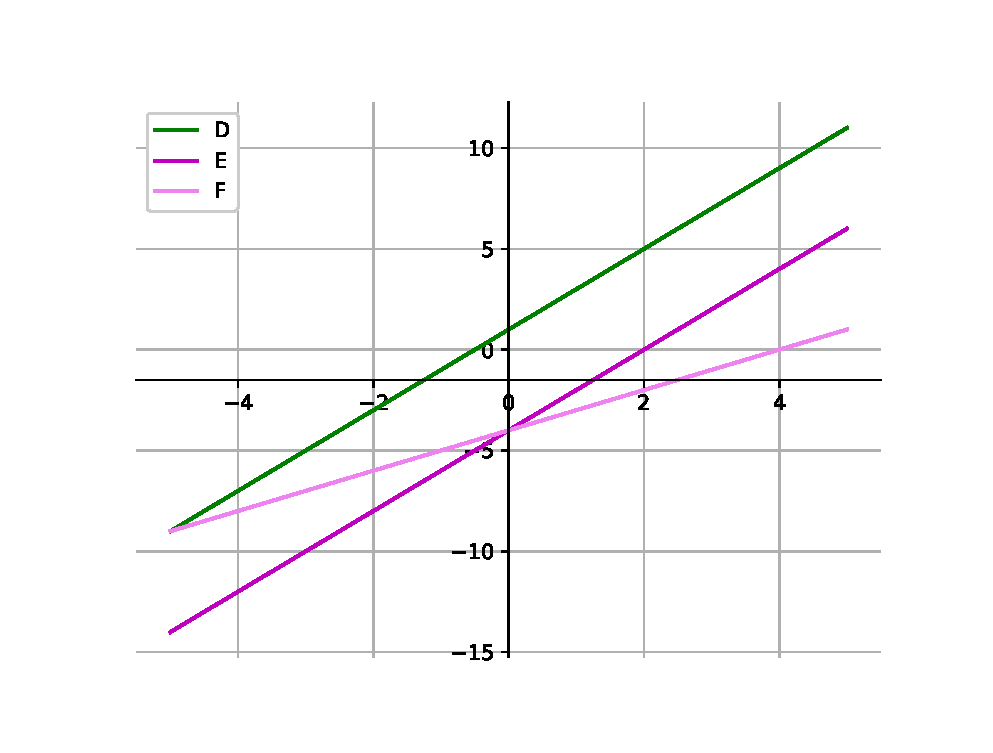
\includegraphics[width=\columnwidth]{./figs/lines/q11b.eps}
	\caption{Lines of Q.3.7.5}
	\label{fig:qelevenb}	
	\end{figure}
		\end{comment}
\end{enumerate}
